\section{Dijkstras algoritme}
\label{dijkstra}

Dijkstras algoritme er en algoritme for å finne korteste vei fra en node til alle andre noder i en urettet graf. Algoritmen er i utgangspunktet for vektede grafer, men kan også anvendes på uvektede. Vi tenker da på en uvektet graf som en vektet graf der alle vektene er like ($ =1 $). Algoritmen er grådig siden vi alltid velger den noden med lavest avstand, og fortsetter derfra. 

\begin{theorem}Dijkstras algoritme

Vi skal finne korteste vei fra en node $ s $ til alle andre noder i en vektet, urettet graf $ G $. 
\begin{enumerate}
\item For alle noder: Sett avstanden fra startnoden $ s $ lik $ \infty $. Sett avstanden fra $ s $ til seg selv lik 0
\item Velg den naboen $ v $ til $ s $ med lavest avstand og marker den som kjent.
\item For hver nabonode $ w $ til $ v $: Dersom avstanden vi får ved å følge veien gjennom $ v $ er kortere enn den gamle avstanden, reduserer vi avstanden fra $ s $ til $ w $, og setter bakoverpekeren i $ w $ til $ v $. 
\end{enumerate}
\end{theorem}


\noindent Vi ser på et eksempel:

\begin{example} Finn korteste vei fra $ v1 $ til alle andre noder:
\begin{figure}[h!]
\centering
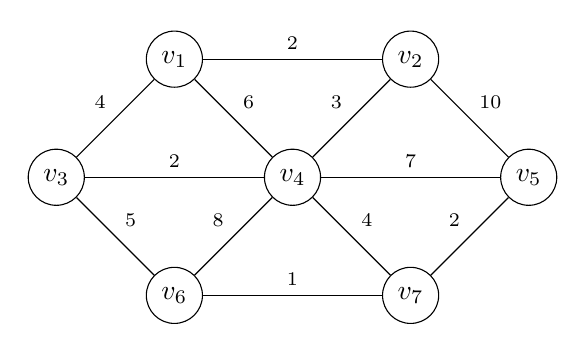
\begin{tikzpicture}[auto,node distance=2cm]
\tikzstyle{vertex} = [circle, draw=black]
\tikzstyle{edge} = [draw=black]

\node[vertex] (v1) at (-1.5,1.5) {$ v_1 $};
\node[vertex] (v2) at (1.5, 1.5) {$ v_2 $};
\node[vertex] (v3) at (-3,0) {$ v_3 $};
\node[vertex] (v4) at (0,0) {$ v_4 $};
\node[vertex] (v5) at (3,0) {$ v_5 $};
\node[vertex] (v6) at (-1.5,-1.5) {$ v_6 $};
\node[vertex] (v7) at (1.5,-1.5) {$ v_7 $};

\draw[edge] (v3) to node{\scriptsize4} (v1);
\draw[edge] (v3) to node{\scriptsize2} (v4);
\draw[edge] (v3) to node{\scriptsize5} (v6);
\draw[edge] (v1) to node{\scriptsize6} (v4);
\draw[edge] (v6) to node{\scriptsize8} (v4);
\draw[edge] (v4) to node{\scriptsize3} (v2);
\draw[edge] (v4) to node{\scriptsize4} (v7);
\draw[edge] (v4) to node{\scriptsize7} (v5);
\draw[edge] (v2) to node{\scriptsize10} (v5);
\draw[edge] (v7) to node{\scriptsize2} (v5);
\draw[edge] (v1) to node{\scriptsize2} (v2);
\draw[edge] (v6) to node{\scriptsize1} (v7);
\end{tikzpicture}
\end{figure}

\noindent Vi begynner med å sette opp en tabell over nodene:
\begin{center}
\begin{tabular}{c | c | c | l}
	 Node   & Kjent & Avstand    & Vei \\ \hline
	$ v_1 $ & T     & 0          & -   \\
	$ v_2 $ & F     & $ \infty $ & -   \\
	$ v_3 $ & F     & $ \infty $ & -   \\
	$ v_4 $ & F     & $ \infty $ & -   \\
	$ v_5 $ & F     & $ \infty $ & -   \\
	$ v_6 $ & F     & $ \infty $ & -   \\
	$ v_7 $ & F     & $ \infty $ & -
\end{tabular}
\end{center}
Vi ser på kantene ut fra $ v_1 $. Vi oppdaterer veien til $ v_2 $, $ v_3 $ og $ v_4 $:
\begin{center}
\begin{tabular}{c | c | c | l}
	 Node   & Kjent & Avstand    & Vei                    \\ \hline
	$ v_1 $ & T     & 0          & -                      \\
	$ v_2 $ & F     & $ 2 $      & $ v_1 \leftarrow v_2 $ \\
	$ v_3 $ & F     & $ 4 $      & $ v_1 \leftarrow v_3 $ \\
	$ v_4 $ & F     & $ 6 $      & $ v_1 \leftarrow v_4 $ \\
	$ v_5 $ & F     & $ \infty $ & -                      \\
	$ v_6 $ & F     & $ \infty $ & -                      \\
	$ v_7 $ & F     & $ \infty $ & -
\end{tabular}
\end{center}
Nå kommer Dijkstras grådige kriterium: Vi velger den noden som har lavest avstand til $ v_1 $ og som ikke er kjent, altså $ v_2 $ og fortsetter derfra. Fra $ v_2 $ har vi kant til $ v_4 $ og $ v_5 $. Ved å gå via $ v_2 $ får vi litt kortere avstand mellom $ v_4 $ og $ v_1 $. Vi oppdaterer tabellen:
\begin{center}
\begin{tabular}{c | c | c | l}
	 Node   & Kjent & Avstand    & Vei                                   \\ \hline
	$ v_1 $ & T     & 0          & -                                     \\
	$ v_2 $ & T     & $ 2 $      & $ v_1 \leftarrow v_2 $                \\
	$ v_3 $ & F     & $ 4 $      & $ v_1 \leftarrow v_3 $                \\
	$ v_4 $ & F     & $ 5 $      & $ v_1 \leftarrow v_2 \leftarrow v_4 $ \\
	$ v_5 $ & F     & $ 12 $     & $ v_1 \leftarrow v_2 \leftarrow v_5 $ \\
	$ v_6 $ & F     & $ \infty $ & -                                     \\
	$ v_7 $ & F     & $ \infty $ & -
\end{tabular}
\end{center}
Neste ukjente node med lavest avstand er $ v_3 $. Vi fortsetter derfra. Vi hopper over et par steg. Slutttabellen ser slik ut:
%\begin{center}
%\begin{tabular}{c | c | c | l}
%	 Node   & Kjent & Avstand    & Vei                                   \\ \hline
%	$ v_1 $ & T     & 0          & -                                     \\
%	$ v_2 $ & T     & $ 2 $      & $ v_1 \leftarrow v_2 $                \\
%	$ v_3 $ & T     & $ 4 $      & $ v_1 \leftarrow v_3 $                \\
%	$ v_4 $ & F     & $ 5 $      & $ v_1 \leftarrow v_2 \leftarrow v_4 $ \\
%	$ v_5 $ & F     & $ 12 $     & $ v_1 \leftarrow v_2 \leftarrow v_5 $ \\
%	$ v_6 $ & F     & $ 9 $      & $ v_1 \leftarrow v_3 \leftarrow v_6 $ \\
%	$ v_7 $ & F     & $ \infty $ & -
%\end{tabular}~~
%\begin{tabular}{c | c | c | l}
%	 Node   & Kjent & Avstand & Vei                                                  \\ \hline
%	$ v_1 $ & T     & 0       & -                                                    \\
%	$ v_2 $ & T     & $ 2 $   & $ v_1 \leftarrow v_2 $                               \\
%	$ v_3 $ & T     & $ 4 $   & $ v_1 \leftarrow v_3 $                               \\
%	$ v_4 $ & T     & $ 5 $   & $ v_1 \leftarrow v_2 \leftarrow v_4 $                \\
%	$ v_5 $ & F     & $ 12 $  & $ v_1 \leftarrow v_2 \leftarrow v_5 $                \\
%	$ v_6 $ & F     & $ 9 $   & $ v_1 \leftarrow v_3 \leftarrow v_6 $                \\
%	$ v_7 $ & F     & $ 9 $   & $ v_1 \leftarrow v_2 \leftarrow v_4 \leftarrow v_7 $
%\end{tabular}
%\end{center}
%
%\begin{center}
%\begin{tabular}{c | c | c | l}
%	 Node   & Kjent & Avstand & Vei                                                  \\ \hline
%	$ v_1 $ & T     & 0       & -                                                    \\
%	$ v_2 $ & T     & $ 2 $   & $ v_1 \leftarrow v_2 $                               \\
%	$ v_3 $ & T     & $ 4 $   & $ v_1 \leftarrow v_3 $                               \\
%	$ v_4 $ & T     & $ 5 $   & $ v_1 \leftarrow v_2 \leftarrow v_4 $                \\
%	$ v_5 $ & F     & $ 12 $  & $ v_1 \leftarrow v_2 \leftarrow v_5 $                \\
%	$ v_6 $ & T     & $ 9 $   & $ v_1 \leftarrow v_3 \leftarrow v_6 $                \\
%	$ v_7 $ & F     & $ 9 $   & $ v_1 \leftarrow v_2 \leftarrow v_4 \leftarrow v_7 $
%\end{tabular}
%\end{center}
%\begin{center}
%\begin{tabular}{c | c | c | l}
%	 Node   & Kjent & Avstand & Vei                                                                 \\ \hline
%	$ v_1 $ & T     & 0       & -                                                                   \\
%	$ v_2 $ & T     & $ 2 $   & $ v_1 \leftarrow v_2 $                                              \\
%	$ v_3 $ & T     & $ 4 $   & $ v_1 \leftarrow v_3 $                                              \\
%	$ v_4 $ & T     & $ 5 $   & $ v_1 \leftarrow v_2 \leftarrow v_4 $                               \\
%	$ v_5 $ & F     & $ 11 $  & $ v_1 \leftarrow v_2 \leftarrow v_4 \leftarrow v_7 \leftarrow v_5 $ \\
%	$ v_6 $ & T     & $ 9 $   & $ v_1 \leftarrow v_3 \leftarrow v_6 $                               \\
%	$ v_7 $ & T     & $ 9 $   & $ v_1 \leftarrow v_2 \leftarrow v_4 \leftarrow v_7 $
%\end{tabular}
%\end{center}
\begin{center}
\begin{tabular}{c | c | c | l}
	 Node   & Kjent & Avstand & Vei                                                                 \\ \hline
	$ v_1 $ & T     & 0       & -                                                                   \\
	$ v_2 $ & T     & $ 2 $   & $ v_1 \leftarrow v_2 $                                              \\
	$ v_3 $ & T     & $ 4 $   & $ v_1 \leftarrow v_3 $                                              \\
	$ v_4 $ & T     & $ 5 $   & $ v_1 \leftarrow v_2 \leftarrow v_4 $                               \\
	$ v_5 $ & T     & $ 11 $  & $ v_1 \leftarrow v_2 \leftarrow v_4 \leftarrow v_7 \leftarrow v_5 $ \\
	$ v_6 $ & T     & $ 9 $   & $ v_1 \leftarrow v_3 \leftarrow v_6 $                               \\
	$ v_7 $ & T     & $ 9 $   & $ v_1 \leftarrow v_2 \leftarrow v_4 \leftarrow v_7 $
\end{tabular}
\end{center}
\end{example}

\subsection{Tidsanalyse}
Hvis vi søker gjennom grafen etter den noden med lavest avstand vil det ta $ O(|V|) $ tid, og dette gjør vi $ |V| $ ganger. Total tid for å finne minste avstand er derfor $ O(|V|^2) $. I tillegg må vi oppdatere avstandene. Det er maksimalt én oppdatering for hver kant, det vil si at det tilsammen tar $ O(|E|) $. Total kjøretid for algoritmen er derfor:
\[ \text{Kjøretid} = |V|^2 + |E| = O\left(|V|^2\right) \]
